\documentclass[letterpaper,oneside]{amsart}
\usepackage[T1]{fontenc}
\usepackage{color,soul}
\usepackage[dvipsnames]{xcolor}
\usepackage[utf8]{inputenc}
\usepackage{amsmath}
\usepackage{amssymb}
\usepackage{tikz}
\usepackage{tikz}
\usepackage{amssymb}

\begin{document}

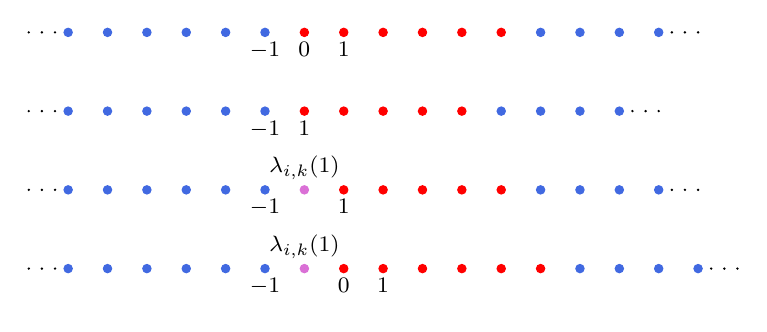
\begin{tikzpicture}
\foreach \x in {-3,...,-1}
	{\filldraw[black] (\x/6,0) circle (0.2pt);}
\foreach \x in {0,...,5}
	{\filldraw[RoyalBlue] (\x/2,0) circle (1.5pt);}
\foreach \x in {0,...,5}
	{\filldraw[Red] (\x/2+6/2,0) circle (1.5pt);}
\foreach \x in {0,...,3}
	{\filldraw[RoyalBlue] (\x/2+12/2,0) circle (1.5pt);}
\foreach \x in {0,...,2}
	{\filldraw[black] (\x/6+15/2+1/6,0) circle (0.2pt);}

\filldraw[black] (5/2,0) circle (0pt) node[anchor=north]{\footnotesize{$-1$}};	
\filldraw[black] (3,0) circle (0pt) node[anchor=north]{\footnotesize{$0$}};
\filldraw[black] (7/2,0) circle (0pt) node[anchor=north]{\footnotesize{$1$}};

\foreach \x in {-3,...,-1}
	{\filldraw[black] (\x/6,-1) circle (0.2pt);}
\foreach \x in {0,...,5}
	{\filldraw[RoyalBlue] (\x/2,-1) circle (1.5pt);}
\foreach \x in {0,...,4}
	{\filldraw[Red] (\x/2+6/2,-1) circle (1.5pt);}
\foreach \x in {0,...,3}
	{\filldraw[RoyalBlue] (\x/2+11/2,-1) circle (1.5pt);}
\foreach \x in {0,...,2}
	{\filldraw[black] (\x/6+14/2+1/6,-1) circle (0.2pt);}

\filldraw[black] (5/2,-1) circle (0pt) node[anchor=north]{\footnotesize{$-1$}};	
\filldraw[black] (3,-1) circle (0pt) node[anchor=north]{\footnotesize{$1$}};

\foreach \x in {-3,...,-1}
	{\filldraw[black] (\x/6,-2) circle (0.2pt);}
\foreach \x in {0,...,5}
	{\filldraw[RoyalBlue] (\x/2,-2) circle (1.5pt);}
\filldraw[Orchid] (6/2,-2) circle (1.5pt);
\foreach \x in {0,...,4}
	{\filldraw[Red] (\x/2+7/2,-2) circle (1.5pt);}
\foreach \x in {0,...,3}
	{\filldraw[RoyalBlue] (\x/2+12/2,-2) circle (1.5pt);}
\foreach \x in {0,...,2}
	{\filldraw[black] (\x/6+15/2+1/6,-2) circle (0.2pt);}

\filldraw[black] (5/2,-2) circle (0pt) node[anchor=north]{\footnotesize{$-1$}};	
\filldraw[black] (3,-2) circle (0pt) node[anchor=south]{\footnotesize{$\lambda_{i,k}(1)$}};
\filldraw[black] (7/2,-2) circle (0pt) node[anchor=north]{\footnotesize{$1$}};

\foreach \x in {-3,...,-1}
	{\filldraw[black] (\x/6,-3) circle (0.2pt);}
\foreach \x in {0,...,5}
	{\filldraw[RoyalBlue] (\x/2,-3) circle (1.5pt);}
\filldraw[Orchid] (6/2,-3) circle (1.5pt);
\foreach \x in {0,...,5}
	{\filldraw[Red] (\x/2+7/2,-3) circle (1.5pt);}
\foreach \x in {0,...,3}
	{\filldraw[RoyalBlue] (\x/2+13/2,-3) circle (1.5pt);}
\foreach \x in {0,...,2}
	{\filldraw[black] (\x/6+16/2+1/6,-3) circle (0.2pt);}

\filldraw[black] (5/2,-3) circle (0pt) node[anchor=north]{\footnotesize{$-1$}};	
\filldraw[black] (3,-3) circle (0pt) node[anchor=south]{\footnotesize{$\lambda_{i,k}(1)$}};
\filldraw[black] (7/2,-3) circle (0pt) node[anchor=north]{\footnotesize{$0$}};
\filldraw[black] (8/2,-3) circle (0pt) node[anchor=north]{\footnotesize{$1$}};
\end{tikzpicture}

\end{document}